\documentclass[a4paper]{tufte-handout}

\title{3. Mass Spectrometry\thanks{Wayne~W.~Z. Yeo}}

\author[ESB]{\textnormal{CHEM 50001} Analytical Chemistry\thanks{Course Instructors: Luke Delmas}}

%\date{28 March 2010} % without \date command, current date is supplied

%\geometry{showframe} % display margins for debugging page layout

\usepackage{graphicx} % allow embedded images
  \setkeys{Gin}{width=\linewidth,totalheight=\textheight,keepaspectratio}
  \graphicspath{{graphics/}} % set of paths to search for images
\usepackage{amsmath,amsthm}  % extended mathematics
\usepackage{physics,siunitx}
\usepackage[version=4]{mhchem}
\usepackage{booktabs} % book-quality tables
\usepackage{units}    % non-stacked fractions and better unit spacing
\usepackage{multicol} % multiple column layout facilities
\usepackage{lipsum}   % filler text
\usepackage{fancyvrb} % extended verbatim environments
  \fvset{fontsize=\normalsize}% default font size for fancy-verbatim environments

% Standardize command font styles and environments
\newcommand{\doccmd}[1]{\texttt{\textbackslash#1}}% command name -- adds backslash automatically
\newcommand{\docopt}[1]{\ensuremath{\langle}\textrm{\textit{#1}}\ensuremath{\rangle}}% optional command argument
\newcommand{\docarg}[1]{\textrm{\textit{#1}}}% (required) command argument
\newcommand{\docenv}[1]{\textsf{#1}}% environment name
\newcommand{\docpkg}[1]{\texttt{#1}}% package name
\newcommand{\doccls}[1]{\texttt{#1}}% document class name
\newcommand{\docclsopt}[1]{\texttt{#1}}% document class option name

\setlength\fboxsep{7px}

\newenvironment{docspec}{\begin{quote}\noindent}{\end{quote}}% command specification environment

\newtheorem{theorem}{Theorem}
\newtheorem{corollary}{Corollary}
\newenvironment{justification} {\begin{proof}[Justification]} {\end{proof}}

\theoremstyle{definition}
\newtheorem{definition}{Definition}
\newtheorem{example}{Example}


\begin{document}

\maketitle% this prints the handout title, author, and date

\begin{abstract}
\noindent
Mass spectrometry is a useful technique for structure determination owing to its sensitivity, where less than a milligram
of substance is required for analysis. Different mass spectrometry techniques and their suitability. High-resolution
mass spectrometry accurately weighs the molecule to give the molecular formula. Analysis of fragmentation patterns.

\end{abstract}

%\printclassoptions

There are different ionisation techniques in mass spectrometry, whether they are fit-for-purpose depends on
different factors, such as the weight and polarity of the sample to be analysed.

\begin{enumerate}
  \item Electron ionisation (EI)
  \item Electrospray ionisation (ESI)
  \item Atmospheric-pressure chemical ionization (APCI)
  \item Matrix-assisted desorption/ionization (MALDI)
\end{enumerate}

\section{Intepreting a mass spectrum}

These principles are most relevant for \textbf{electron ionisation} mass spectrometry, where we expect
extensive fragmentation of analyte molecules.

\begin{enumerate}
  \item Find out \textbf{what reagents and solvents} have been used in the reaction. Especially if this
  is a crude mass spectrum, starting material and byproducts do tend to appear.
  \item Identify the \textbf{molecular ion} and base peak.
\end{enumerate} 

\section{Electrospray ionisation \textnormal{(ESI)}}
\section{Atmospheric-pressure chemical ionization \textnormal{(APCI)}}
\section{Matrix-assisted desorption/ionization \textnormal{(MALDI)}}

\newthought{Electronic spectra are incredibly complex}, due to the stimulation of simultaneous vibrational and rotational
transitions. But why are electronic transitions so strongly coupled to nuclear motion?

When an electronic transition occurs, the nuclei are inevitably subjected to a change in electrostatic force, due to the
redistribution of electronic charge. The \textbf{potential energy surface}, which governs nuclear motion, changes as a
direct result of electronic transitions.

As a result, the nuclei respond by breaking into vibration to arrive at their new equilibrium geometry. Simultaneous
electronic and vibrational transitions are \textbf{vibronic transitions}.

\section{Selection Rules}

There are two selection rules governing electronic transitions, which can be expressed as various parts of the\marginnote{g/u formally only apply to
molecules which are centrosymmetric.}
term symbol. $$\Delta S = 0 \quad \Delta \Lambda = 0 \pm 1$$
$$ \ce{g} \not\rightarrow \ce{g} \quad \ce{u} \not\rightarrow \ce{u} \quad \ce{g} \rightarrow \ce{u}$$

The spin selection rule $\Delta S = 0$ means \textbf{singlet-triplet transitions are forbidden}. If heavy atoms are
\marginnote{In \ce{I2} the forbidden \ce{^3\Pi}--\ce{^1\Sigma} transition is responsible for the brown colour of iodine vapour.}present,
the spin selection rule begins to break down due to spin-orbit coupling.
%\begin{justification}
%  Can add a justification here one day.
%\end{justification}

In general, \textbf{allowed electronic transitions must involve a change in symmetry}. \cite{atkins2014atkins}

\section{The Frank-Condon Principle}

\begin{definition}[Fermi's Golden Rule] Describes the rate of a photophysical event $k$.
  \begin{equation}
    k(\mathrm{s}^{-1}) = \frac{2\pi}{h} \mathrm{FC} \times \mathrm{V}^2
  \end{equation}
  where FC is the \textbf{Franck-Condon factor}: probability that nuclei are in a position where an \textit{isoenergetic} electronic transition is possible.
  \marginnote{Isoenergetic states are important, that is where electron transfer can occur due to quantum tunnelling}
  The \ce{V^2} term is \textbf{electronic coupling}: rate of electronic transition.


\end{definition}

\begin{definition}[Frank-Condon Principle]\marginnote{These electronic transitions can take place in different contexts: 1. change of electron orbital (electron transfer) or 2. absorption of photon (photochemistry)}
  Because nuclear masses are so much larger than the mass of an electron, an electronic transition occurs
  within a stationary framework. \textbf{The nuclear wavefunction remains unchanged during an electronic transition}.
\end{definition}

We can now use this principle to develop a framework to predict and explain the vibrational transitions.

\begin{theorem}[Franck-Condon Principle] The intensity of a particular vibrational transition depends on the Franck–Condon factor.

  \begin{justification}
    The intensity of a transition between electronic states $i$ and $j$ depends on the population of the lower state $i$ (Boltzmann)
    and the square of the transition dipole moment $\boldsymbol{\mu}_{ji}$.

    \begin{equation*}
      \boldsymbol{\mu}_{ji} = \int \psi_i^* \hat{\mu} \psi_j \mathrm{d} \tau
    \end{equation*}

    In this integral, $\hat{\mu}$ is the dipole moment operator, representing the interaction between the light
    and the molecule.

    Using the Born-Oppenheimer approximation, the wavefunctions can be written as a product of a wavefunction 
    which depends only on the electrons $\psi_{\mathrm{el}}$ and a wavefunction which depends only on the \marginnote{convenient separation of variables}
    vibrational motion of the nuclei $\psi_{\mathrm{vib}}$.

    \begin{equation*}
      \boldsymbol{\mu}_{ji} = \int \psi_{\mathrm{el}}'^* \psi_{\mathrm{vib},i} \hat{\mu} \psi_{\mathrm{el}}'' \psi_{\mathrm{vib,}j} \mathrm{d} \tau
    \end{equation*}
    In this expression we have used ' and '' to denote the initial and final electronic states, and have used i and j to indicate vibrational 
    levels in the two electronic states. The vibrational wavefunctions are real, so the $^*$ has been dropped.

    For an electronic transition we can assume that the relevant part of the dipole moment operator does not affect the vibrational wavefunctions, and
    integral can be separated into two parts (relying on the Franck-Condon Principle).

    \begin{equation*}
      \boldsymbol{\mu}_{ji} = \left[ \int\psi_{\mathrm{vib},i} \psi_{\mathrm{vib,}j}\mathrm{d}r  \right] \times  \left[\int \psi_{\mathrm{el}}'^* \hat{\mu} \psi_{\mathrm{el}}'' \mathrm{d}\tau \right] 
    \end{equation*}
    For the vibrational term, the integration is over the internuclear separation $r$.
    
    The quantity in the right-hand square brace is the electronic \marginnote{$\hat{\mu}$ is antisymmetric, which affects the symmetry of allowed electronic transitions.}
    transition moment, whose value is determined by the electronic states. If the transition is forbidden, this integral will be zero.

    \begin{definition}[Franck-Condon factor]
      \begin{equation*}
        q_{i,j} = \left[ \int\psi_{\mathrm{vib},i} \psi_{\mathrm{vib,}j}\mathrm{d}r  \right]^2
      \end{equation*}
      
    \end{definition}

    The quantity in the left-hand square brace is simply the \textit{overlap integral} between the vibrational wavefunctions. The square of this quantity is known 
    as the Franck-Condon factor, and it is important in determining the intensity of transitions between different vibrational energy levels.

   

  \end{justification}

  The Franck-Condon factor will be largest when there is good overlap between two vibrational wavefunctions, which in practice means that the principal maxima
  of the wavefunctions should be aligned.
  
\end{theorem}

Qualitatively, the transition occurs from the ground vibrational state of the lower electronic state to the vibrational state 
that it most resembles in the upper electronic state. In that way, the vibrational wavefunction undergoes \textbf{least change} in an electronic transition, 
which corresponds to the preservation of the dynamical state of the nuclei as required by the Franck-Condon Principle (Definition 2).

\begin{marginfigure}
  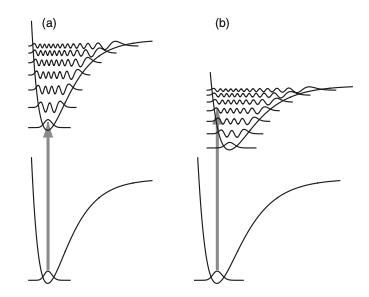
\includegraphics[width=55mm]{fcprinciple.png}
  \caption{PE curves for absorption. (a) the two PE curves are aligned, so the strongest transition in the absorption spectrum will be $0 \rightarrow 0$. (b)
  the upper state is displaced to the right, now the $0 \rightarrow 0$ but the later members of the vibronic progression ($0 \rightarrow 1$, $0 \rightarrow 2$) will have significant intensity.} 
\end{marginfigure}

If the equilibrium geometry of \ce{S1} is similar to the equilibrium geometry of \ce{S0}, there is only a small displacement in potential
energy surfaces and the $0 \rightarrow 0$ transition is strongest.



\subsection{Summary}

\begin{enumerate}
  \item Allowed electronic transitions must involve a symmetry change.
  \item The transition dipole moment is a one-electron operator.
  \item Allowed electronic transitions preserve spin.
  \item Electronic transitions are always accompanied by vibrational transitions. [Franck-Condon Principle]
\end{enumerate}

\section{Fluorescence}

\subsection*{Kinetics: differential and integral rate laws}

\begin{equation}
  \frac{\mathrm{d}[\ce{S}_1]}{\mathrm{d}t} = -(k_R +k_{IC} +k_{ISC}) [\ce{S}_1]
\end{equation}

\begin{equation}
[\ce{S}_1]_t = [\ce{S}_1]_0 \exp[-(k_R + k_{IC} + k_{ISC})t]
\end{equation}

Hence, with a steady state approximation we have the following relation:
\begin{equation}\label{eq:1}
\mathbf{\Phi}_F = \frac{k_R}{k_R + k_{IC} + k_{ISC}} = \frac{k_R}{k_0} = \frac{\tau_0}{\tau_R}
\end{equation}

The sum of $(k_R + k_{IC} + k_{ISC})$, which is $1/\tau_0$, can be measured from the decay of fluorescence.
Taking this with a measure of $\Phi_F$ enable us to use Equation \ref{eq:1} to find $k_R$.

\section{Phosphorescence}

Phosphorescence typically has a longer lifetime ($10^{-4} \mathrm{s}$) because singlet-triplet transitions are spin forbidden, so the spontaneous
emission rate $k_P$ is slower than that for a singlet-singlet transition (fluorescence, $k_R$). The population of excited triplet states \ce{T}
is built up by \textbf{intersystem crossing}.

\subsection*{Intersystem Crossing (ISC)}
Intersystem crossing is possible due to \textbf{spin-orbit coupling}: the coupling of electron spin
with orbital angular momentum. This is encouraged by heavy atoms (Br, I) which give rise to strong spin-orbit coupling and fast ISC.\marginnote{$V_{SO}$ is proportional to the fourth power of nuclear charge.}

ISC is also enhanced with a large Franck-Condon factor, which increases the probability of the singlet and triplet state having vibrational levels which are
isoenergetic.
\begin{itemize}
  \item Large, flexible molecules (lots of dense vibrational modes)
  \item Polar environments, through polar solvents and macromolecules
  \item Small energy gap between $\ce{S1}$ and $\ce{T1}$ (less electronic energy lost to vibrational)
\end{itemize}

\subsection*{Triplet Formation Quantum Yield}

A quantum yield for ISC can be defined in a similar way to that for fluorescence.

$$\mathbf{\Phi}_T = \frac{k_{ISC}}{k_0}$$

\subsection*{Internal Conversion (IC)}

As the name suggests, internal \textit{conversion} refers to the isoenergetic conversion of electronic energy to vibrational energy
between two electronic states of the \textit{same} multiplicity.

IC between $\ce{S1}$ and $\ce{S0}$ involves very highly excited vibrational levels of $\ce{S0}$. After IC, vibrational relaxation would
quickly take the molecule down to to lower vibrational levels of $\ce{S0}$.

\textbf{IC is fast from higher electronic excited states} due to a smaller energy gap from $\ce{S2} \rightarrow \ce{S1}$ etc. Therefore, most
molecules rapidly relax to $\ce{S1}$ through IC. 

\section{Unimolecular Photochemistry}

Reactions involving a single molecule, not requiring an additional collision provided by diffusion. For example,

\begin{enumerate}
  \item Ionisation: $\ce{A^*} \rightarrow \ce{A+} + \ce{e-}$
  \item Unimolecular dissociation: $\ce{A^{*}} \rightarrow \ce{B} + \ce{C}$
  \item Isomerisation: $\ce{A^*} \rightarrow \ce{A}'$
\end{enumerate}

\subsection*{Kinetics}
Unimolecular photochemistry is apparent as an additional first order reaction pathway with a rate $k_{PC}$, which follows
the first-order rate law $\nu_{\mathrm{uni}} = k_{PC}[\ce{A^*}]$. Therefore, the total rate constant $k$ is now a
sum of both photophysical ($k_0$) and photochemical ($k_{PC}$) rates of decay.
\begin{align*}
  k &= k_R + k_{ISC} + k_{IC} +k_{PC} \\
    &= k_0 + k_{PC}
\end{align*}

Unimolecular photochemistry can be observed as quenching of fluorescence, which results in a reduction of emission lifetime and quantum yield,
as shown below.
\begin{equation}
  \tau_0' = \frac{1}{k_0 + k_{PC}} \qquad \phi_f' = \frac{k_R}{k_0 + k_{PC}}
\end{equation}

And this is how the fluorescence quantum yields are related in the presence and absence of photochemistry -- they are directly proportional to each other.
$$\frac{\phi_F'}{\phi_F} = \frac{\tau_0'}{\tau_0}$$

From the above relations, we can arrive at the \textbf{photochemical quantum yield} $\phi_{PC}$ and \textbf{photochemical rate constant} $k_{PC}$.

\begin{align}
  \phi_{PC} &= \frac{k_{PC}}{k_0 + k_{PC}} = 1 - \frac{\phi_F'}{\phi_F} \\
  k_{PC} &= k_R \left( \frac{1}{\phi_F'} - \frac{1}{\phi_F}\right) = \frac{1}{\tau_o'}- \frac{1}{\tau_0}
\end{align}

\section{Bimolecular Photochemistry}

Bimolecular reactions involving a collision between two molecules, resulting in electron or energy transfer. For example,
\marginnote{Bimolecular photochemistry typically involves triplet states due to longer excited state lifetimes.}

\begin{enumerate}
  \item Quenching: $\ce{^1A^*} + \ce{Q} \rightarrow \ce{A} + \ce{Q}$
  \item Electron transfer: $\ce{^1A^*} + \ce{B} \rightarrow \ce{A+} + \ce{B-}$
  \item Addition: $\ce{^1A^*} + \ce{B} \rightarrow \ce{AB}$
\end{enumerate}

In the following examples, we will largely look at \textbf{quenching} to exemplify bimolecular photochemistry.
Different molecules show different quenching efficiencies: we know that species with unpaired electrons (\ce{O2}) and easily polarisable atoms 
(e.g. I) are particularly good at quenching electronically excited states.

\subsection*{Kinetics}

The example reactions provided above all share a second-order rate law $\nu_{\mathrm{bi}} = k_{Q}[\ce{^1A^*}][\ce{Q}]$.
\marginnote{Or it can be that $[\ce{Q}] \gg [\ce{^1A^*}]$ which results in pseudo first-order kinetics as well.}
If we can assume the quencher is not consumed, $[\ce{Q}]$ remains constant, and the process is pseudo first-order with rate constant $k_Q[\ce{Q}]$. The
pseudo first-order rate law is
\begin{equation}
  [\ce{^1A^*}_1]_t = [\ce{^1A^*}_1]_0 \exp \{ -(k_R + k_{IC} + k_{ISC} + k_Q[\ce{Q}])t \}
\end{equation}

From the definition of $\phi_F$, the quenched fluorescence quantum yield $\phi_F'$ is a function of $[\ce{Q}]$.

\begin{equation}
  \phi_F' = \frac{k_R}{k_0 + k_Q[\ce{Q}]}
\end{equation}

Thus, after some steady-state approximation,

\begin{equation}
  \frac{\phi_{F}}{\phi_{F}'} = \frac{\tau_0}{\tau_0'} = \frac{k_0 + k_Q[Q]}{k_0} = 1 + \frac{k_Q}{k_0}[\ce{Q}]
\end{equation}

The ratio $\phi_F / \phi_F'$ can be developed into a useful result, referred to as \textbf{Stern-Volmer Analysis}.

\begin{align*}
  \frac{\phi_F}{\phi_F'} &= \frac{k_R}{k_R + k_{IC} + k_{ISC}} \frac{k_R + k_{IC} + k_{ISC} + k_Q[\ce{Q}]}{k_R} \\
  &= \frac{k_R}{k_0} \frac{k_0 + k_Q[\ce{Q}]}{k_R} \\
  &= 1 + \frac{k_Q[\ce{Q}]}{k_0} \\
  &= 1 + \tau_0 k_Q[\ce{Q}]
\end{align*}

\begin{marginfigure}
  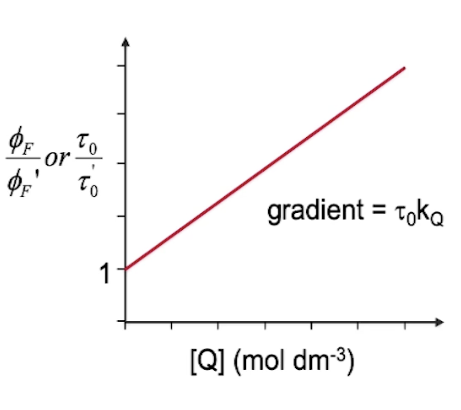
\includegraphics[width=48mm]{stern_volmer.png}
  \caption{Stern-Volmer plot} 
\end{marginfigure}

A Stern-Volmer  plot of $\phi_F/\phi_F'$ against [\ce{Q}] will give a straight line of slope $\tau_0 k_Q$.

\section{Fluorescence Resonance Energy Transfer}

If the emission spectrum of one molecule significantly overlaps with the absorption spectrum of another molecule,
\marginnote{This process is mediated by a direct interaction (dipole-dipole coupling) between two molecules, and is not photon transfer.}and
if both molecules are in \textit{close proximity}, there can be efficient \textbf{non-radiative energy transfer} from the first molecule
(the donor) to the second (the acceptor). When the absorption and emission spectra overlap, there is a probability of isoenergetic energy 
levels that exist betwen donor and acceptor
(Franck-Condon Factor).

\begin{equation}
  \ce{FC} \propto J = \int I_{S*} \epsilon_Q \mathrm{d} v
\end{equation}
where the normalised overlap integral J is determined by the overlap of donor emission ($I_{S*}$) and acceptor absorption ($\epsilon_Q$) spectra.

The fluorescence resonance energy transfer efficiency is given by

\begin{equation}
  \phi_{\ce{FRET}} = \frac{k_{\ce{FRET}}}{k_{\ce{FRET}}+k_0} = \frac{R_0^6}{R_0^6+R_{DA}^6}
\end{equation}

where $R_{DA}$ is the distance between donor and acceptor and \marginnote{$R_0$ is defined such that $R_{DA} = R_0$, $k_{FRET} = k_0.$ The rate of FRET is equal that of other photophysical processes, energy transfer efficiency $\phi_{FRET} = 0.5$.}
$$k_{\ce{FRET}} = k_0 \left( \frac{R_0}{R_{DA}} \right)^6 \quad R_0= C\left( \frac{\kappa^2 \phi_D J}{n^4}\right)^{1/6}$$

As we can see in the above relation, the efficiency of FRET is highly dependent on distance (tens of nm).

\subsection*{Quenching of donor emission is evidence of FRET}

We can typically observe FRET as quenching of donor emission, which can be unimolecular or bimolecular. 

\begin{itemize}
  \item Efficient FRET between a donor and acceptor results in quenching of donor emission and increase in acceptor emission.
  \item Inefficient FRET between a donor and acceptor results in emission of both donor and acceptor being observed.
\end{itemize}

\subsection*{Summary}

\begin{itemize}
  \item FRET is non-radiative energy transfer between two molecules.
  \item Adheres to the Fermi Golden Rule.
  \item Efficient FRET requires \textbf{1.} good overlap between acceptor and donor energy levels (FC) \textbf{2.} good dipole-dipole coupling ($\ce{V^2}$) and \textbf{3.} close proximity (rate $\propto 1/R^6$).
  \item Typical range of donor-acceptor separation is up to 10 nm.
\end{itemize}


\section{Electron Transfer}

The rate of electron transfer $k_{ET}$ has a strong distance and medium dependence.\marginnote{This is due to the V factor, which represents electronic interaction based on spatial overlap of donor
and acceptor wavefunctions.}
\begin{equation}
  k_{ET} \propto \ce{V^2} \propto \exp(-\beta r)
\end{equation}
where r is the distance, and $\beta$ depends on the property of the medium between donor and acceptor.

\begin{itemize}
  \item $\beta = 0$ \si{\angstrom}$^{-1}$ are delocalised systems, which provide pathways for very efficient electron transport.
  \item $\beta = 0.7$ \si{\angstrom}$^{-1}$ are systems linked via rigid covalent bonds (molecular wires) which can transport electrons with a chain rich in electrophilic nuclei.
  \item $\beta = 1.4 - 2.8$ \si{\angstrom}$^{-1}$ Solvent and vacuum aren't that great for electron transfer.
\end{itemize}

Because electron transfer through quantum tunnelling must be isoenergetic, thermal excitation is required\marginnote{FC factor, which gives rise to energy dependence of electron transfer.}
to reach the crossing point. This is the \textbf{activation barrier}.

\begin{figure}
  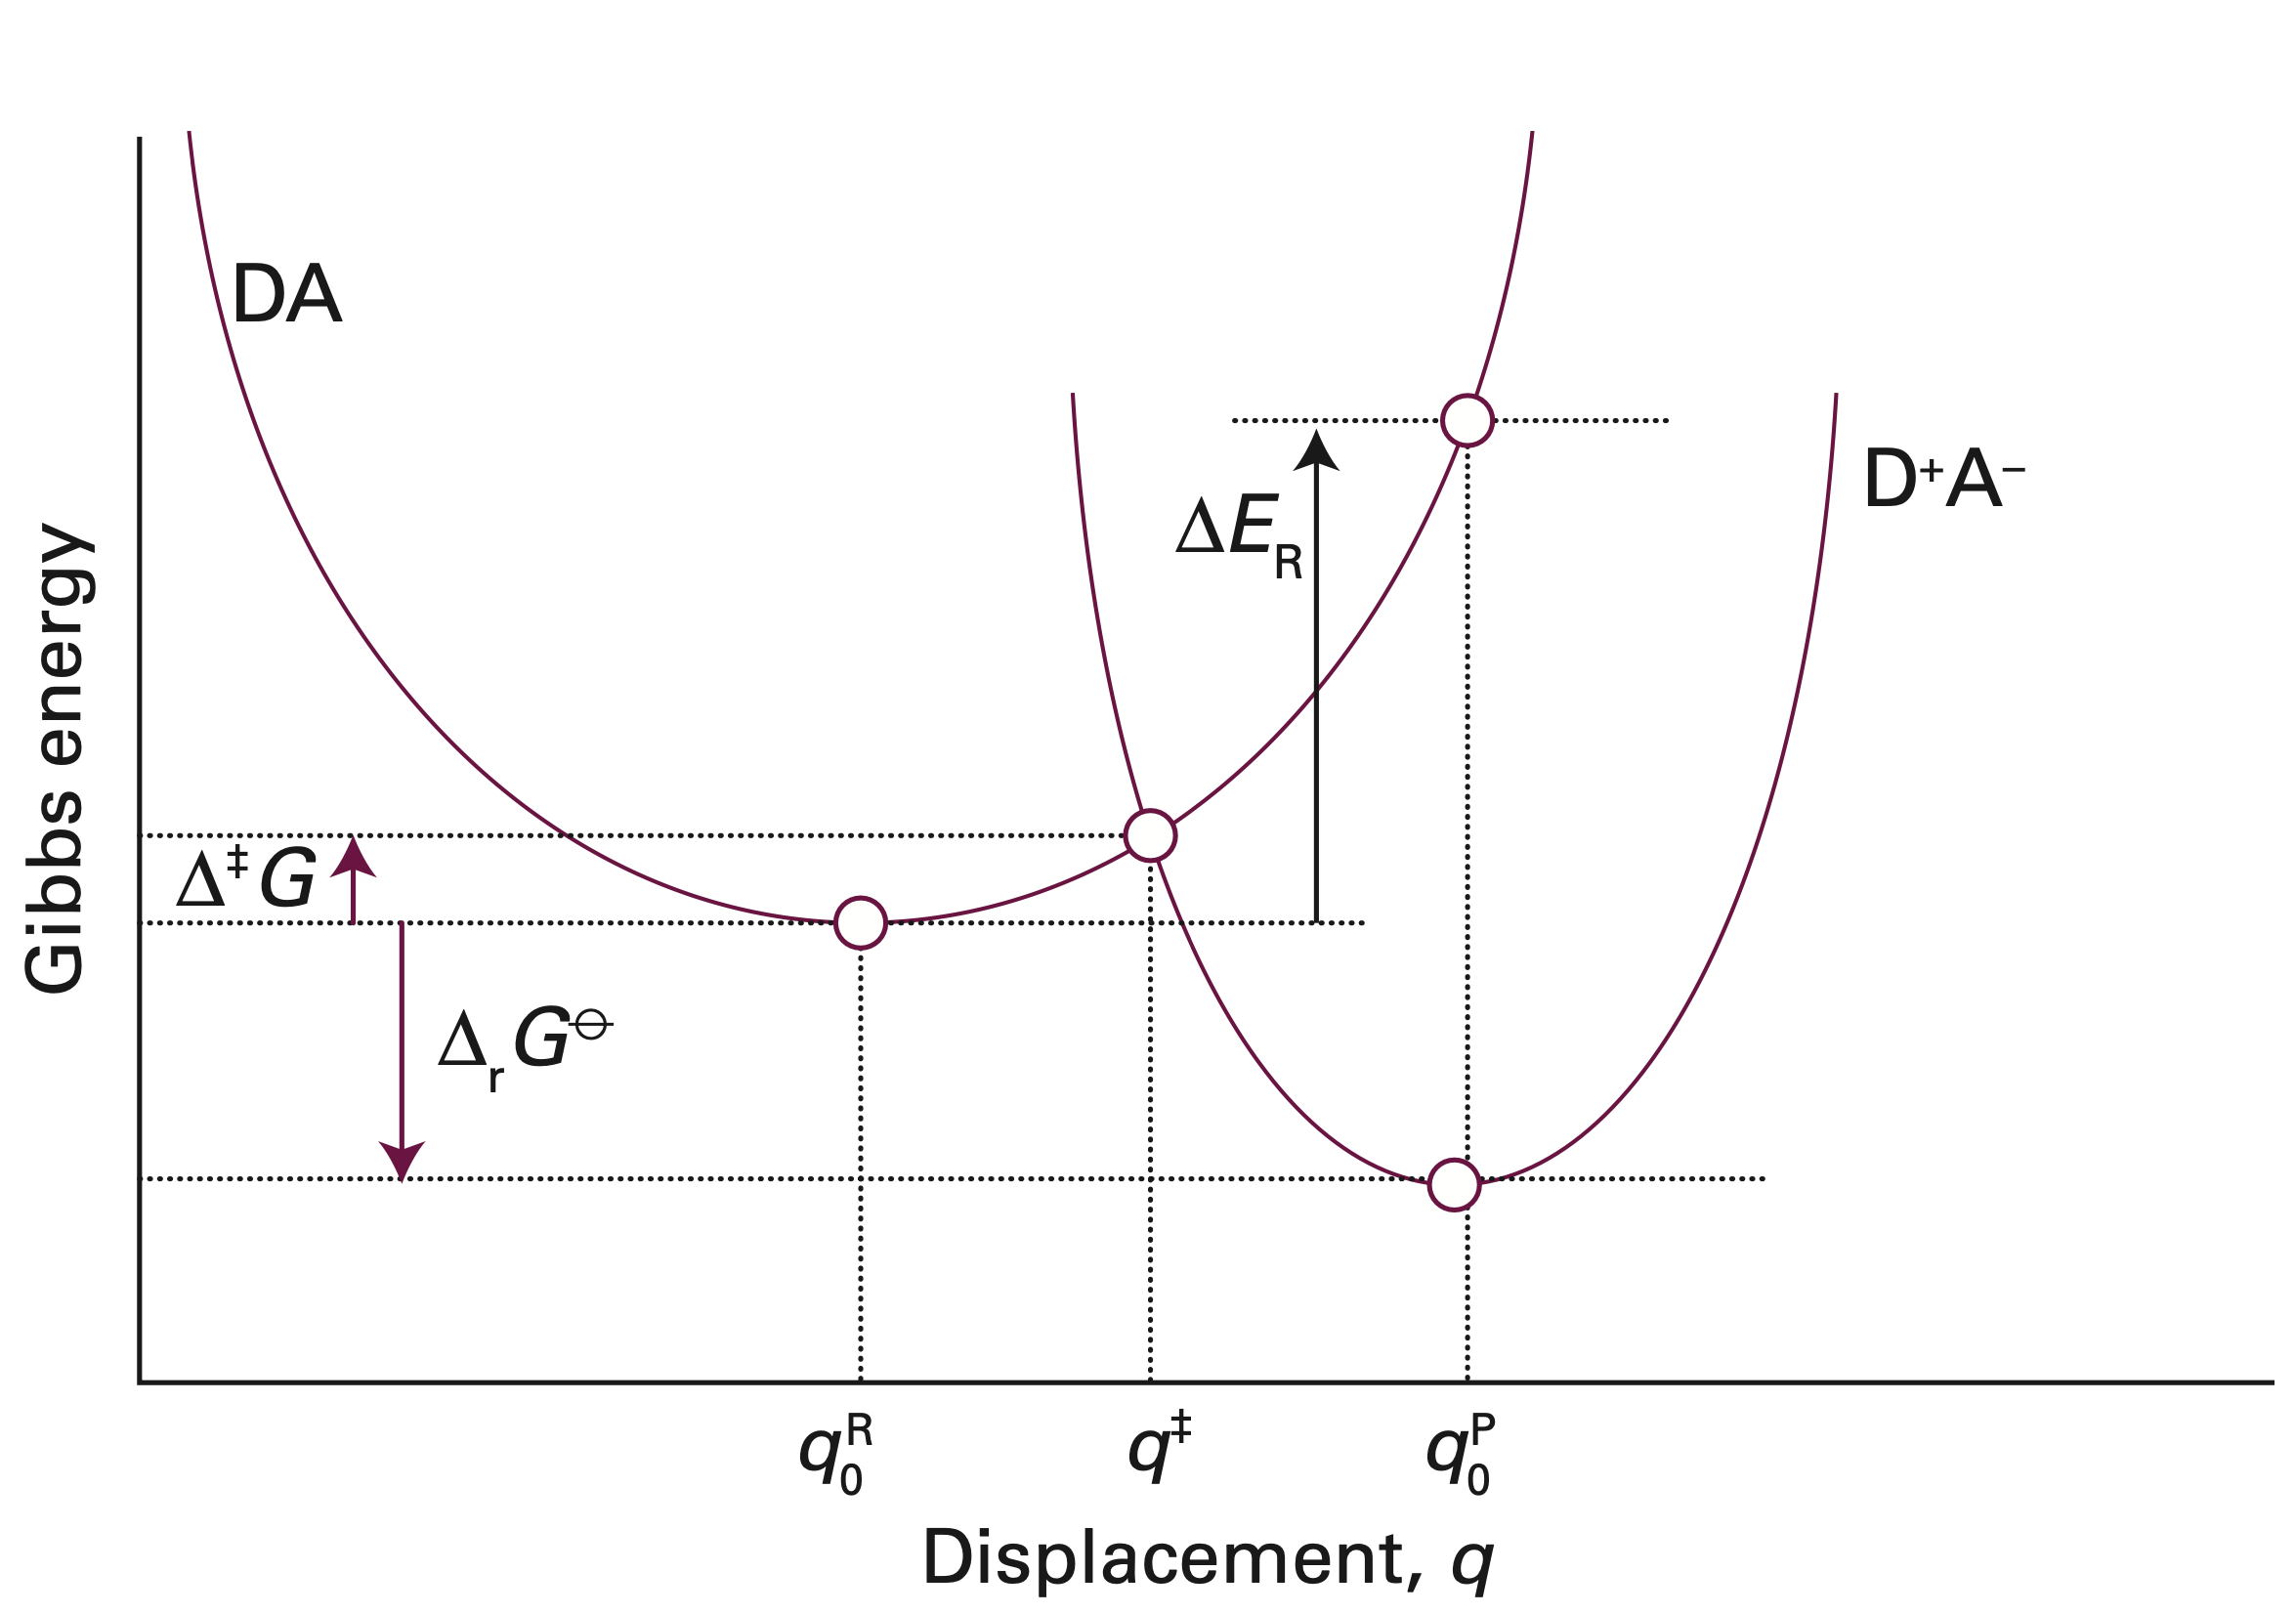
\includegraphics[width=100mm]{ET_pes.png}
  \caption{Gibbs energy surfaces of \ce{DA} amd \ce{D+A-} involved in a typical electron transfer process represented as simple harmonic oscillators.
  $q_0^R$ and $q_0^P$ are equilibrium structures of reactant and product.} 
\end{figure}

\marginnote{$\lambda$ is the reorganization energy, the energy change associated with the molecular rearrangement for DA to take the equilibrium geometry of \ce{D+A-}.}
\begin{equation}
  k_{ET} \propto \ce{FC^2} \propto \exp \left( \frac{\Delta G^{\ddag}}{k_B T} \right) = \exp \left( \frac{(\Delta G^{0} + \lambda)^2}{4 \lambda k_B T} \right)
\end{equation}


In unimolecular donor-acceptor systems, the above relation can be used in conjunction with
\begin{equation*}
  k_{PC} = k_R \left( \frac{1}{\phi_F'} - \frac{1}{\phi_F}\right) = \frac{1}{\tau_o'}- \frac{1}{\tau_0}
\end{equation*}

\subsection*{Summary}

\begin{itemize}
  \item Electron transfer is distance dependent to maximise the spatial orbital overlap.
  \item Electron transfer is energy dependent due to the isoenergetic condition of quantum tunnelling.
\end{itemize}

\bibliography{photochem}
\bibliographystyle{plainnat}



\end{document}
